\section{Exact solutions for simple cases}\label{sec:exactSolutions}

In PHS form, the Hubbard Hamiltonian may then be written as a sum of kinetic, chemical and potential energy terms, respectively:

\begin{equation}\label{eq:hubbard}
\mathcal{H} = \mathcal{H}_K + \mathcal{H}_\mu + \mathcal{H}_V ,
\end{equation}
defined as

\begin{equation}\label{eq:def_energies}
\begin{split}
\mathcal{H}_K &= -t \sum_{\left\langle i, j \right \rangle, \sigma} ( c_{i,\sigma} c_{j,\sigma}^\dagger + c_{j,\sigma}^\dagger c_{i,\sigma} ) \\
\mathcal{H}_\mu &= -\mu \sum_i ( n_{i,\uparrow} + n_{i,\downarrow} ) \\
\mathcal{H}_V &= U \sum_{i} ( n_{i,\uparrow} - \frac{1}{2} ) ( n_{i,\downarrow} - \frac{1}{2} )
\end{split} ,
\end{equation}
where:

\begin{itemize}
\item $i$ and $j$ label sites on the lattice.
\item $c_{i,\sigma}^{(\dagger)}$ is an operator that annihilates (creates) an electron with spin $\sigma$ on site $i$.
\item $n_{i,\sigma}$ is the number operator counting the number of electrons of spin $\sigma$ on site $i$ (either 0 or 1).
\item $t$ is the hopping parameter related to the kinetic energy of the electrons. It is determined by the overlap of the atomic wave functions on neighboring sites $\left\langle i, j \right\rangle$.
\item $U$ is the repulsive Coulomb interaction between electrons on the same lattice site. Whenever a site $i$ has two electrons, there is a local repulsion between them corresponding to an energy cost $U n_{i \uparrow} n_{i \downarrow}$. The constant $1/2$ terms serve to recast the Hamiltonian in particle-hole symmetric form.
\item $\mu$ is the chemical potential controlling the electron number (or density).
\end{itemize}

A given physical observable of interest $\mathcal{O}$, such as the spin-spin correlation, or the magnetic susceptibility may be computed formally by

\begin{equation}
\left\langle \mathcal{O} \right\rangle = \text{Tr} ( \mathcal{O} \mathcal{P} )
\end{equation}
where

\begin{equation}\label{eq:projection}
\mathcal{P} \equiv \frac{1}{Z} e^{-\beta \mathcal{H} } , \text{ with } Z = \text{Tr} ( e^{-\beta \mathcal{H} } )
\end{equation}

The trace is taken over the Hilbert space corresponding to all possible configurations of the lattice occupation. Defining an orthonormal basis of this Hilbert space $\{ | \psi_\alpha \rangle | \alpha = 1, ... D \} $, where $D$ is the dimension of the Hilbert space, the partition function reads

\begin{equation}\label{eq:z_asEigen}
\Tr ( e^{-\beta \mathcal{H} } )= \sum_\alpha \left\langle \psi_\alpha | e^{-\beta \mathcal{H} } | \psi_\alpha \right\rangle
\end{equation}

There are four possible states at each site in the Hubbard model: $\left| \,\, \right\rangle$, $\left|\uparrow \right\rangle$, $\left|\downarrow\right \rangle$, $\left|\uparrow \downarrow \right\rangle $, corresponding, respectively, to no electron, a spin up or spin down electron, and two electrons of opposite spin occupying the site. The potential energy operator acts as follows

\begin{equation}
U (n_{i\uparrow} - \frac{1}{2} ) ( n_{i\downarrow} - \frac{1}{2} ) 
\begin{cases}
\left| \,\, \right\rangle = \frac{U}{4} \left| \,\, \right\rangle \\
\left|\uparrow \right\rangle = -\frac{U}{4} \left|\uparrow \right\rangle \\
\left|\downarrow\right \rangle = -\frac{U}{4} \left|\downarrow\right \rangle \\
\left|\uparrow \downarrow \right\rangle = \frac{U}{4} \left|\uparrow \downarrow \right\rangle \\
\end{cases}
\end{equation}

Singly occupied states ($\left|\uparrow \right\rangle$, $\left|\downarrow\right \rangle$) have lower energy and are thus more likely to occur. They correspond to nonzero magnetization $m = n_{\uparrow} - n_{\downarrow}$, which is favored by the Hubbard interaction $U$. A relevant question is whether or not the spins order in space when $t \neq 0$ and to what extent.

Let us now establish our notations for second quantized operators to introduce a different representation of electronic states on the lattice. The fermionic annihilation and creation operators anticommute.

\begin{equation}
\{ c_{j\sigma} , c_{l \sigma'}^\dagger \} = \delta_{jl} \delta_{\sigma\sigma'}
\end{equation}

The $c$-operator algebra is further defined by the vanishing of all other anticommutators.

\begin{equation}\label{eq:fermion_anticom}
\{ c_{j\sigma}^{(\dagger)} , c_{l \sigma'}^{(\dagger)} \} = 0
\end{equation}

Note that taking $l = j$ and $\sigma = \sigma'$ in equation (\ref{eq:fermion_anticom}) for the $c^\dagger$-operators, we recover Pauli's exclusion principle since $(c_{j\sigma}^\dagger)^2 = 0$. If we omit the site $i$ and spin $\sigma$ indices, a convenient way of specifying states on the lattice is

\begin{equation}
\begin{split}
&\left| 0 \right\rangle : \text{unoccupied state - no electron} \\
&\left| 1 \right\rangle : \text{occupied state - one electron}
\end{split}
\end{equation}
so that a generic state may be written as a product of the states above $\otimes_{i=1}^{N} \otimes_{\sigma = \pm 1/2} \left| n \right\rangle_{i, \sigma}$ at each site for each spin state, where $n= 0, 1$. For example, one such state is

\begin{equation}
\left| 0 \right\rangle_{1, 1/2} \left| 1 \right\rangle_{1, -1/2} \left| 0 \right\rangle_{2, 1/2} \left| 0 \right\rangle_{2, -1/2} ... \left| 0 \right\rangle_{N, 1/2} \left| 1 \right\rangle_{N, -1/2}  ,
\end{equation}
where $N$ is the number of sites on the lattice.

The creation and annihilation operators act as follows

\begin{equation}
c \left| 0 \right\rangle = 0 \quad c^\dagger \left| 0 \right\rangle = \left| 1 \right\rangle \quad c \left| 1 \right\rangle = \left| 0 \right\rangle \quad c^\dagger \left| 1 \right\rangle = 0
\end{equation}

Thus, the eigenstates of the number operator are $\left| 0 \right\rangle, \left| 1 \right\rangle$:

\begin{equation}
n \left| 0 \right\rangle = 0 \quad n \left| 1 \right\rangle = \left| 1 \right\rangle
\end{equation}

Moreover, the operator $c_i^\dagger c_{i+1}^\dagger$, corresponding to the hopping from site $i+1$ to $i$, i.e. to the kinetic energy of the electrons on neighboring sites, acts as follows (ignoring spin):

\begin{equation}
c_i^\dagger c_{i+1}^\dagger \begin{cases}
\left|0 0 \right\rangle = 0 \\
\left|1 0 \right\rangle =  0 \\
\left|0 1 \right\rangle =  \left| 1 0 \right\rangle \\
\left|1 1 \right\rangle =  c_i^\dagger \left| 1 0  \right\rangle = 0 \\
\end{cases}
\end{equation}

The operator annihilates the particle at $i+1$ and creates it back at $i$, i.e. the electron hops from $i+1$ to $i$.

\subsection{The purely atomic $\frac{t}{U} = 0$ limit}

When $t = 0$, the site index may be omitted since the Hamiltonian is a sum of operators solely at site $i$. Hence, we have $[ \mathcal{H}, n_{i,\sigma} ] = 0 \forall i $, and the eigenstates of $\mathcal{H}$ are also eigenstates of all number operators at the different sites in the lattice. Thus, in the single site limit, we obtain

\begin{equation}
\mathcal{H} = U (n_\uparrow - \frac{1}{2} ) (n_\downarrow - \frac{1}{2} ) - \mu ( n_\uparrow + n_\downarrow )
\end{equation}
which acts as follows (using the eigenstates of $n_\sigma$)

\begin{equation}
\mathcal{H} \begin{cases}
\left| \,\, \right\rangle = \frac{U}{4} \\
\left| \uparrow \right\rangle = \bigg( \frac{U}{4} - (\mu + \frac{U}{2} ) \bigg) \left| \uparrow \right\rangle \\
\left| \downarrow \right\rangle = \bigg( \frac{U}{4} - (\mu + \frac{U}{2} ) \bigg) \left| \downarrow \right\rangle \\
\left| \uparrow \downarrow \right\rangle = \bigg( \frac{U}{4} - 2 \mu \bigg) \left| \uparrow \downarrow \right\rangle
\end{cases}
\end{equation}

Thus, the Hamiltonian is diagonal in the basis $\{\left| \psi_\alpha \right\rangle \} = \left| \,\, \right\rangle, \left|\uparrow \right\rangle, \left|\downarrow\right \rangle, \left|\uparrow \downarrow \right\rangle $:

\begin{equation}
\begin{split}
&\bigg[ \mathcal{H}_{\rho\gamma} \bigg] = \bigg[ \left\langle \psi_\rho \left| \mathcal{H} \right| \psi_\gamma \right\rangle \bigg] \\
&= \text{diag}\bigg(\frac{U}{4}, \frac{U}{4} - (\mu + \frac{U}{2} ), \frac{U}{4} - (\mu + \frac{U}{2} ), \frac{U}{4} - 2 \mu \bigg) ,
\end{split}
\end{equation}
which means that $e^{-\beta \mathcal{H} }$ is also diagonal:

\begin{equation}
e^{-\beta \mathcal{H} } = e^{-\beta U / 4}  \text{diag}\bigg(1,  e^{\beta(\mu + \frac{U}{2})}, e^{\beta(\mu + \frac{U}{2})},  e^{2\beta \mu} \bigg)
\end{equation}
and this is one of the rare situations in which it is possible to explicitly write down a closed form for the partition function.

\begin{equation}
\begin{split}
Z &= \text{Tr} ( e^{-\beta\mathcal{H} } ) = \sum_\alpha \left\langle \psi_\alpha \left|e^{-\beta \mathcal{H} } \right| \psi_\alpha \right\rangle \\
&= e^{-\beta U / 4} \bigg(1 + 2 e^{\beta(\mu + \frac{U}{2})} + e^{2 \beta \mu} \bigg)
\end{split}
\end{equation}

Moreover, some of the observables that were mentioned before are explicitly computable. This is because due to the diagonal form of $\mathcal{H}$, the expressions defining these observables greatly simplify.

\begin{equation}
\begin{split}
\mathcal{H} e^{-\beta\mathcal{H} } &\mapsto e^{-\beta U / 4}  \text{diag}\bigg(\frac{U}{4}, (-\mu - \frac{U}{4})  e^{\beta(\mu + \frac{U}{2})} (-\mu - \frac{U}{4}) e^{\beta(\mu + \frac{U}{2})}, (\frac{U}{4} - 2\mu ) e^{2\beta \mu} \bigg) \\
n_{\uparrow} e^{-\beta\mathcal{H} } &\mapsto e^{-\beta U / 4}  \text{diag}\bigg(0, e^{\beta(\mu + \frac{U}{2})}, 0,  e^{2\beta \mu} \bigg) \\
n_{\downarrow} e^{-\beta\mathcal{H} } &\mapsto e^{-\beta U / 4}  \text{diag}\bigg(0, 0, e^{\beta(\mu + \frac{U}{2})},   e^{2\beta \mu} \bigg) \\
n_{\uparrow} n_{\downarrow} e^{-\beta\mathcal{H} } &\mapsto e^{-\beta U / 4}  \text{diag}\bigg(0, 0, 0,   e^{2\beta \mu} \bigg) \\
\end{split}
\end{equation}

From these we can compute some traces which we shall find useful to obtain averages of various observables.

\begin{equation}
\begin{split}
&\Tr \bigg( \mathcal{H} e^{-\beta\mathcal{H} } \bigg) = e^{-\beta U / 4} \bigg(\frac{U}{4} + 2 (-\mu - \frac{U}{4})  e^{\beta(\mu + \frac{U}{2})} + (\frac{U}{4} - 2\mu ) e^{2\beta \mu} \bigg) \\
&\Tr \bigg( (n_\uparrow + n_\downarrow ) e^{-\beta\mathcal{H} } \bigg) = e^{-\beta U / 4} \bigg(2 (-\mu - \frac{U}{4})  e^{\beta(\mu + \frac{U}{2})} + (\frac{U}{4} - 2\mu ) e^{2\beta \mu} \bigg) \\
&\Tr \bigg( n_\uparrow n_\downarrow \bigg) = e^{-\beta U/4} e^{2\beta\mu}
\end{split}
\end{equation}

The bottom line is that we are able to obtain \emph{exact} expressions for

\begin{enumerate}
\item the one-site density $\rho = \left\langle n_\uparrow \right\rangle + \left\langle n_\downarrow \right\rangle$, measuring the average occupation of each site.
\begin{equation}
\begin{split}
\rho &= \frac{\text{Tr} \big[ (n_\uparrow + n_\downarrow ) e^{-\beta\mathcal{H}} \big]}{Z} \\
&= \frac{2 e^{\beta(\frac{U}{2} + \mu)} + 2 e^{2\beta\mu}}{1 + 2 e^{\beta(\mu + \frac{U}{2})} + e^{2 \beta \mu}}
\end{split}
\end{equation}

Note that when there is no chemical potential $\mu = 0$, we have $\rho = 1$ for any $U$, or $\beta$. This corresponds to half filling: the density of electrons is half its maximum possible value.

\begin{figure}[H]
	\centering
\hspace{12mm}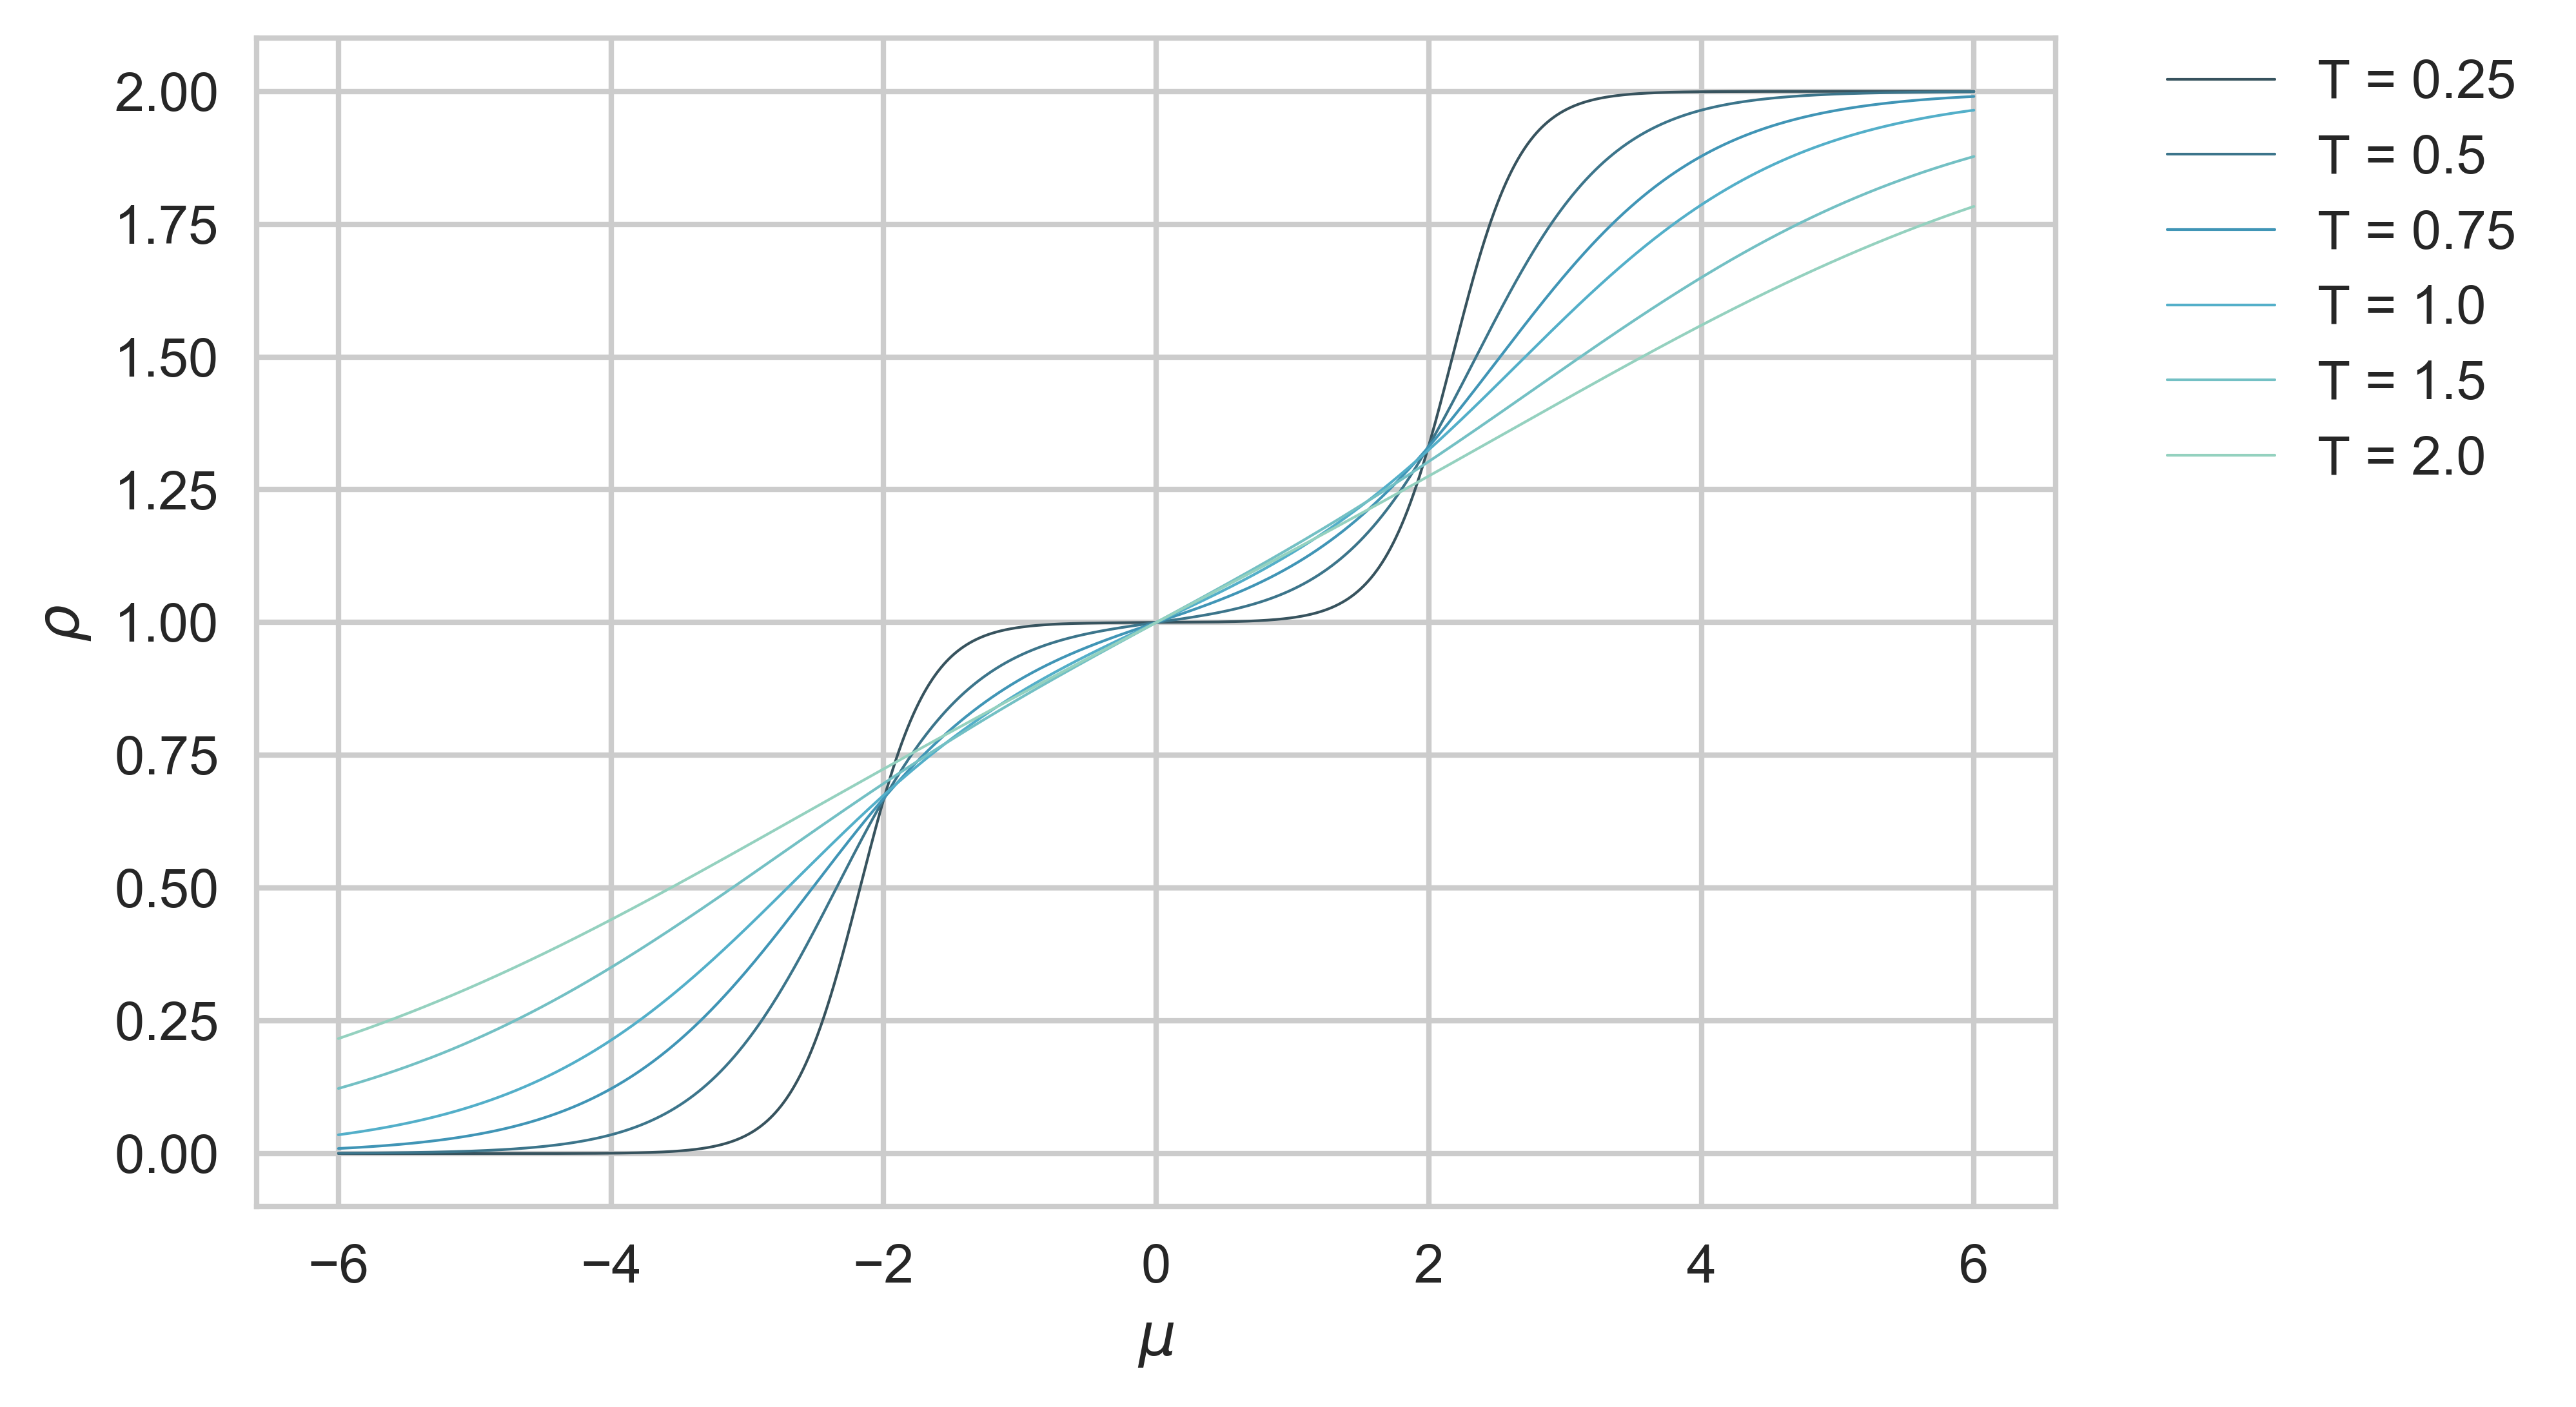
\includegraphics[width=0.83\linewidth]{Figures/HubbardModel/rhoVsMu.png}
	\caption[]{}
	\label{fig:rhoVsMu}
\end{figure}

\item the one-site energy $E = \left\langle \mathcal{H} \right\rangle$.
\begin{equation}
\begin{split}
E &= \frac{\text{Tr}\bigg( \mathcal{H}e^{-\beta\mathcal{H} } \bigg)}{Z} \\
&= \frac{ \frac{U}{4} + 2 ( -\mu - \frac{U}{4} ) e^{\beta(\frac{U}{2} + \mu )} + (\frac{U}{4} - 2\mu ) e^{2\beta\mu}}{1 + 2 e^{\beta (\frac{U}{2} + \mu )} + e^{2\beta\mu} } \\
&= \frac{ \frac{U}{4} ( 1 + 2 e^{\beta (\frac{U}{2} + \mu )} + e^{2\beta\mu} )}{1 + 2 e^{\beta (\frac{U}{2} + \mu )} + e^{2\beta\mu} } + \frac{2(-\mu - \frac{U}{4}) e^{\beta(\frac{U}{2} + \mu)} - 2\mu e^{2\beta\mu} - 2\frac{U}{4} e^{\beta (\frac{U}{2} + \mu)} }{1 + 2 e^{\beta (\frac{U}{2} + \mu )} + e^{2\beta\mu}} \\
&= \frac{U}{4} - \frac{ (2\mu - U) e^{\beta(\frac{U}{2} + \mu) } + 2\mu e^{2\beta\mu} }{1 + 2 e^{\beta (\frac{U}{2} + \mu )} + e^{2\beta\mu} }
\end{split}
\end{equation}
which at half filling becomes

\begin{equation}
E = \frac{U}{4} - \frac{U}{2 ( 1 + e^{-\beta U /2} )}
\end{equation}

\item the double occupancy $\left\langle n_\uparrow n_\downarrow \right\rangle$.

\begin{equation}
\left\langle n_\uparrow n_\downarrow \right\rangle = \frac{\text{Tr} \big[ n_\uparrow n_\downarrow \big]}{Z} = \frac{e^{2\beta\mu}}{1 + 2 e^{\beta (\frac{U}{2} + \mu )} + e^{2\beta\mu}}
\end{equation}
which, at half filling, simplifies to

\begin{equation}
\left\langle n_\uparrow n_\downarrow \right\rangle = \frac{1}{2 ( 1 + e^{\beta U/2} )}
\end{equation}

Note that as either $U$ or $\beta$ increase the double occupancy tends to zero.
\end{enumerate}

\subsection{The non-interacting $\frac{t}{U} \rightarrow \infty$ limit}

In the $\frac{t}{U} \rightarrow \infty$ limit, the spin spaces become independent, and they may be considered separately. Thus, we omit the spin indices of the operators in the Hamiltonian:

\begin{equation}
\mathcal{H} = -t \sum_{\left\langle i, j \right\rangle} \big( c_i^\dagger c_j + c_j^\dagger c_i \big) - \mu \sum_i n_i
\end{equation}
which may be recast as a bilinear form

\begin{equation}
\mathcal{H} = \bm c^\dagger ( -t \bm K - \mu \bm I ) \bm c ,
\end{equation}
where

\begin{equation}
\bm c = \bigg[ c_1 \,\, c_2 \,\, ... \,\, c_N \bigg]^T \quad \bm c^\dagger = \bigg[c_1^\dagger \,\, c_2^\dagger \,\, ... c_N^\dagger \bigg]
\end{equation}
and $\bm I$ is the identity matrix. We also defined a matrix of zeros and ones specifying the hopping geometry, $\bm K$. When writing down $\bm K$, we must specify the boundary conditions. Periodic boundary conditions (PBCs) preserve a system's translational invariance and are advantageous because they reduce finite size effects. An example of a quantity which is measured more accurately is energy. In the thermodynamic limit, $N \rightarrow \infty$, the measured energy differs from the actual value by a correction of order $\mathcal{O}(\frac{1}{N^2})$ with PBCs \textcolor{red}{missing citation}, while for open boundary conditions (OBCs), the correction is of order $\mathcal{O}(\frac{1}{N})$. Additionally, PBCs have the property of giving site independent observables. For example, the electron density per site does not vary with PBCs, but it varies with the distance to the edges of the lattice when we use OBCs.

Consider a rectangular two-dimensional lattice with $N_x \times N_y$ sites. Then, we have $\dim(\bm K) = N_x N_y \times N_x N_y $, and

\begin{equation}
\bm K = \bm I_y \otimes \bm K_x + \bm I_x \otimes \bm K_y ,
\end{equation}
where $\bm I_{x, y}$ are identity matrices of dimension $N_{x, y}$, respectively, and $\bm K_{x, y}$ are the hopping matrices in the $x$ and $y$-directions respectively.

For lattices in 1D or 2D, it is possible to find an exact eigendecomposition

\begin{equation}
\bm K = \bm F^T \bm \Lambda \bm F \quad \text{with}  \quad \bm F^T \bm F = \bm I ,
\end{equation}
where $\bm \Lambda = \text{diag}(\lambda_k)_{k = 1}^{N_x N_y}$ is a diagonal matrix of eigenvalues of $\bm K$. The Hamiltonian is diagonalized:

\begin{equation}\label{eq:quadraticH}
\mathcal{H} =\tilde{\bm c}^\dagger \big( -t \bm K - \mu \bm I \big) \tilde{\bm c} = \sum_k \varepsilon_k \tilde{n}_k ,
\end{equation}
where $\tilde{\bm c} = \bm F \bm c$ and $\tilde{\bm c}^\dagger = (\bm F \bm c)^\dagger$, and

\begin{equation}
\varepsilon_k = -t \lambda_k - \mu \quad \tilde{n}_k = \tilde{c}_k^\dagger \tilde{c}_k
\end{equation}

The $\tilde{c}$-operators are equally valid electron creation/annihilation operators, obeying the same anticommutation relations as the original operators $c_i$. While the original operators create/annihilate particles at specific (spatial) sites, the new ones create/annihilate particles with momentum $k$. Both sets of operators describe the same physics, however the interaction term in the Hubbard model is fairly complex to write in momentum space so it is not possible to apply this procedure to diagonalize it.

\bigskip

Now, it turns out that it is easy to evaluate the partition function for quadratic Hamiltonians. If $\mathcal{H} = \bm c^\dagger \bm H \bm c$, where $\bm H$ is a $N \times N$ Hermitian matrix, then we have that

\begin{equation}\label{eq:trace_quadratic}
\text{Tr} \big[ e^{-\beta \mathcal{H} } \big] = \prod_{i=1}^N ( 1 + e^{-\beta \lambda_{k_i} } ) ,
\end{equation}
where $\lambda_{k_i}$ are the eigenvalues of $\bm H$.

We present a proof of this result in appendix \ref{ap:Zquadratic}.

Thus, this result suggests that if we are able to devise some approximation to transform the quartic term of the interacting Hubbard model in a quadratic form, then we can solve it.

To complete the solution of the non-interacting case we apply the result of equation (\ref{eq:trace_quadratic}) to compute the partition corresponding to the quadratic Hamiltonian defined in equation (\ref{eq:quadraticH}):

\begin{equation}
Z = \prod_k ( 1 + e^{-\beta \varepsilon_k} )
\end{equation}

Now that we have found a closed form solution for $Z$, it is again possible to find closed form expressions for observables of interest as well, namely:

\begin{enumerate}
\item the density, or average occupation of each site, $\rho$.

\begin{equation}
\rho = \left\langle n \right\rangle = \left\langle \tilde{n} \right\rangle = \frac{1}{N} \sum_{k=1}^N \left\langle \tilde{n}_k \right\rangle  = \frac{1}{N} \sum_{k=1}^N  \frac{1}{1 + e^{\beta\varepsilon_k}}
\end{equation}

\item the energy $E = \left\langle \mathcal{H} \right\rangle$.

\begin{equation}
E = \frac{1}{N} \sum_k \frac{\varepsilon_k}{1 + e^{\beta\varepsilon_k}}
\end{equation}

\item the equal-time Green's function, which plays a key role in computing other quantities, such as correlation functions.

\begin{equation}
G_{lj} = \left\langle c_l c_j^\dagger \right\rangle = \frac{1}{N} \sum_k e^{ i k \cdot ( l - j ) } ( 1 - f_k ),
\end{equation}
where $f_k = \big(1 + e^{\beta(\varepsilon_k - \mu)} \big)^{-1}$ is the Fermi-Dirac distribution (of course, here we consider half filling: $\mu = 0$). Note that the Green function, like the Hamiltonian, is translationally invariant: $G_{lj} = G_{l-j}$. If we use PBCs, no site is singled out, they are all equivalent and this behavior of the Green's function should become apparent.
\end{enumerate}